\section{Additional Experiments}

Finally, we present the results of the experiments with the MLP architecture in \Cref{apx:fig:experiments-mlp}. We observe that the MLP architecture underperforms compared to the Transformer architecture. Nonetheless, \fname{} often outperforms PPO and generally performs on par with SHAC.

Interestingly, the Discovery scenario appears to be the most challenging, as none of the algorithms (PPO and \fname{}) are able to make any meaningful progress. This may be caused by the sample inefficiency of the MLP architecture, combined with the fact that the world model cannot access the full state.

The only scenario where SHAC outperforms \fname{} is the Transport scenario. This may be due to the MLP's inability to overcome the gradient noise from the world model.

\begin{figure}[t]
    \centering
    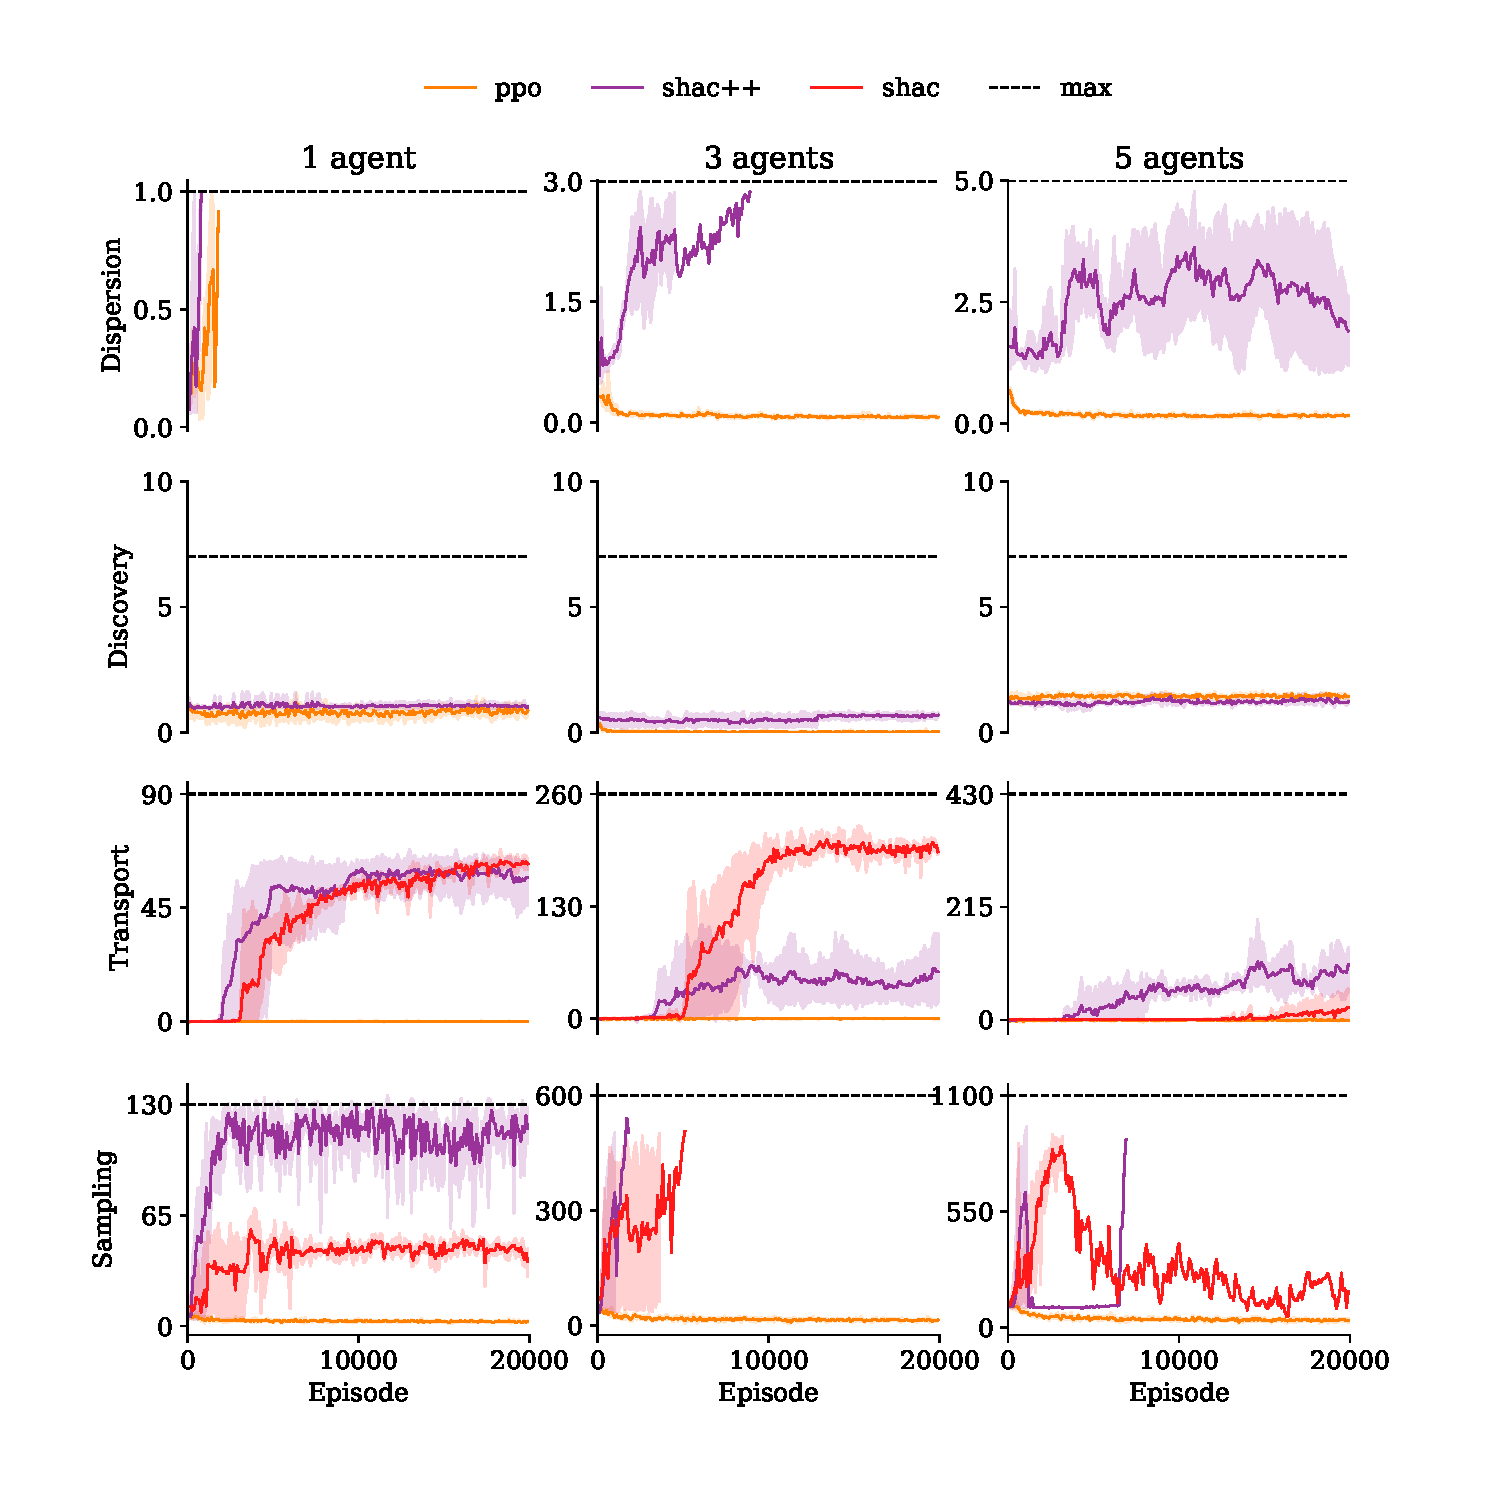
\includegraphics[width=\columnwidth]{figs/main-mlp.pdf}
    \caption{Comparison between \fname{}, PPO, and SHAC for increasing number of agents for Dispersion, Transport, Discovery, and Sampling scenarios with the MLP architecture.
    We show the mean and standard deviation of the normalized rewards across $3$ runs. For the MLP architecture see \Cref{fig:experiments}.
    }
    \label{apx:fig:experiments-mlp}

\end{figure}


